\documentclass[mingoth,11pt,a4j,uplatex]{jsarticle}
\usepackage[top=20truemm,bottom=20truemm,left=20truemm,right=20truemm]{geometry}
\usepackage{moreverb}
\usepackage{listings,jlisting} %日本語のコメントアウトをする場合jlistingが必要
								% https://qiita.com/N_Matsukiyo/items/1199f07a0e1bf4fce29c
\usepackage[dvipdfmx]{graphicx}
 
% https://qiita.com/ta_b0_/items/2619d5927492edbb5b03
\lstset{
  basicstyle={\ttfamily},
  identifierstyle={\small},
  commentstyle={\smallitshape},
  keywordstyle={\small\bfseries},
  ndkeywordstyle={\small},
  stringstyle={\small\ttfamily},
  frame={tb},
  breaklines=true,
  columns=[l]{fullflexible},
  numbers=left,
  xrightmargin=0zw,
  xleftmargin=3zw,
  numberstyle={\scriptsize},
  stepnumber=1,
  numbersep=1zw,
  lineskip=-0.5ex
}


\renewenvironment{description}%  descriptionをインデント
{%
   \begin{list}{\parbox{1zw}{$\bullet$}}% 見出し記号/直後の空白を調節
   {%
      \setlength{\topsep}{1zh}
      \setlength{\itemindent}{3zw}
      \setlength{\leftmargin}{5zw}%  左のインデント
      \setlength{\rightmargin}{0zw}% 右のインデント
      \setlength{\labelsep}{1zw}%    黒丸と説明文の間
      \setlength{\labelwidth}{3zw}%  ラベルの幅
      \setlength{\itemsep}{0em}%     項目ごとの改行幅
      \setlength{\parsep}{0em}%      段落での改行幅
      \setlength{\listparindent}{0zw}% 段落での一字下り
   }
}{%
   \end{list}%
}

\title{Face Recognition First Step}
\author{小林 統 \thanks{帝京平成大学現代ライフ学部人間文化学科メディア文化コース}}
\date{\today}

\setcounter{secnumdepth}{3}
\setcounter{tocdepth}{3}

\begin{document}
%\gtfamily	%全てゴシックに

\maketitle

\begin{abstract}
顔認識ライブラリclmtrackr.js を利用して、SNOWアプリを作ってみよう。
\end{abstract}

\tableofcontents
\newpage

\section{はじめに}
\subsection{読み間違えないでね}

\begin{lstlisting}[caption=読み間違えないでね]
数字:0123456789
小文字:abcdefghijklmnopqrstuvwxyz
大文字:ABCDEFGHIJKLMNOPQRSTUVWXYZ

1:イチ
l:小文字のエル
i:小文字のアイ
!:ビックリマーク
|:バーティカルバー。Shiftと¥を押したもの。

0:ゼロ
o:小文字のオー
O:大文字のオー

.:ピリオド
,:コンマ
\end{lstlisting}

\subsection{注意}
\begin{itemize}
\item これから出てくるソースコードには、左に「行番号」と呼ばれる番号が出てくるけど、入力する必要ないからね。

\item scriptタグの中で「//」で始まる文は、コメントで、プログラムは読み飛ばすよ。

\item コピーできるところはコピーして効率よく入力して行こう
\item 徐々に追加されていくから、量が多く見えるけど、平気だよ!
\item 改行されていても、行番号が書かれていないところは、1行だからね。表示上改行されて見えてるだけ
\end{itemize}

\newpage
\section{07-01.html ブラウザからカメラの情報を取得しよう}
\small
まずは、カメラの映像をホームページに写してみよう。

\begin{lstlisting}[caption=07-01.html]
<!DOCTYPE html>
<html lang="ja">
    <head>
        <meta charset="utf-8">
        <meta name="viewport" content="width=device-width,initial-scale=1">
        <title>顔認識</title>
        <style>
            /* video 要素の上に canvas 要素をオーバーレイするための CSS */
            /* コンテナ用の div について */
            #container {              
                position: relative;   /* 座標指定を相対値指定にする */
            }
            /* カメラ映像を流す video について */
            #video {                  
                transform: scaleX(-1);/* 左右反転させる */
            }
        </style>
    </head>

    <body>
        <!-- video の上に canvas をオーバーレイするための div 要素 -->
        <div id="container">  
            <!-- カメラ映像を流す video -->
            <video id="video" width="400" height="300" autoplay></video>
        </div>
        <script>
            // もろもろの準備
            var video = document.getElementById("video");   // video 要素を取得
            // getUserMedia によるカメラ映像の取得
            var media = navigator.mediaDevices.getUserMedia({// メディアデバイスを取得
                video: {facingMode: "user"},                          
                // カメラの映像を使う
                audio: false                                          
                // マイクの音声は使わない
            });
            media.then((stream) => {// メディアデバイスが取得できたら
              video.srcObject = stream;
            });

        </script>
    </body>
</html>
\end{lstlisting}

\newpage
\section{07-02.html 顔の特徴となる点を取得しよう}
clmtrackr.jsを用いて、顔の特徴となる点を取得しよう。緑色の線で顔の輪郭や眉・目・鼻・口の位置を特定するよ。
これは、あらかじめ多くの写真で学習させたモデルmodel\_pca\_20\_svm.jsがあるからできるよ。

\begin{lstlisting}[caption=07-02.html]
<!DOCTYPE html>
<html lang="ja">
    <head>
        <meta charset="utf-8">
        <meta name="viewport" content="width=device-width,initial-scale=1">
        <title>顔認識</title>
        <style>
            /* video 要素の上に canvas 要素をオーバーレイするための CSS */
            /* コンテナ用の div について */
            #container {              
                position: relative;   /* 座標指定を相対値指定にする */
            }
            /* カメラ映像を流す video について */
            #video {                  
                transform: scaleX(-1);/* 左右反転させる */
            }
            #canvas {                 /* 描画用の canvas について */
                transform: scaleX(-1);  /* 左右反転させる */
                position: absolute;     /* 座標指定を絶対値指定にして */
                left: 0;                /* X座標を0に */
                top: 0;                 /* Y座標を0に */
            }
        </style>
    </head>

    <body>
        <!-- video の上に canvas をオーバーレイするための div 要素 -->
        <div id="container">  
            <!-- カメラ映像を流す video -->
            <video id="video" width="400" height="300" autoplay></video>
            <!-- 重ねて描画する canvas -->
            <canvas id="canvas" width="400" height="300"></canvas>        
        </div>
        
        <!-- clmtrackr 関連ファイルの読み込み -->
        <script src="js/clmtrackr.js"></script>          <!-- clmtrackr のメインライブラリの読み込み -->
        <script src="js/model_pca_20_svm.js"></script>   <!-- 顔モデル(※)の読み込み -->
        
        <script>
            // もろもろの準備
            var video = document.getElementById("video");   // video 要素を取得
            var canvas = document.getElementById("canvas"); // canvas 要素の取得
            var context = canvas.getContext("2d");          // canvas の context の取得
            
            // getUserMedia によるカメラ映像の取得
            var media = navigator.mediaDevices.getUserMedia({// メディアデバイスを取得
                video: {facingMode: "user"},                          
                // カメラの映像を使う
                audio: false                                          
                // マイクの音声は使わない
            });
            media.then((stream) => {// メディアデバイスが取得できたら
              video.srcObject = stream;
            });
            
            // clmtrackr の開始
            var tracker = new clm.tracker();  // tracker オブジェクトを作成
            tracker.init(pModel);             // tracker を所定のフェイスモデル(※)で初期化
            tracker.start(video);             // video 要素内でフェイストラッキング開始

            // 描画ループ
            function drawLoop() {
                requestAnimationFrame(drawLoop);                      // drawLoop 関数を繰り返し実行
                var positions = tracker.getCurrentPosition();         // 顔部品の現在位置の取得
                context.clearRect(0, 0, canvas.width, canvas.height); // canvas をクリア
                tracker.draw(canvas);                                 // canvas にトラッキング結果を描画
            }
            drawLoop();                                             // drawLoop 関数をトリガー
            

        </script>
    </body>
</html>
\end{lstlisting}

\newpage
\section{07-03.html 特徴となる点を数値で見てみよう}
clmtrackr.jsで取得された点の配列を数値として表示してみよう。

\vspace{1em}
\begin{center}
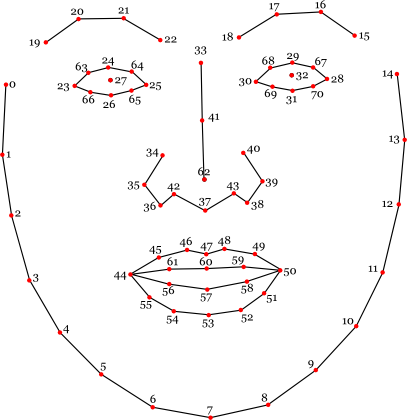
\includegraphics[width=5cm]{img/facemodel_numbering_new.png}
\end{center}

\begin{lstlisting}[caption=07-03.html]
<!DOCTYPE html>
<html lang="ja">
    <head>
        <meta charset="utf-8">
        <meta name="viewport" content="width=device-width,initial-scale=1">
        <title>顔認識</title>
        <style>
            /* video 要素の上に canvas 要素をオーバーレイするための CSS */
            /* コンテナ用の div について */
            #container {              
                position: relative;   /* 座標指定を相対値指定にする */
            }
            /* カメラ映像を流す video について */
            #video {                  
                transform: scaleX(-1);/* 左右反転させる */
            }
            #canvas {                 /* 描画用の canvas について */
                transform: scaleX(-1);  /* 左右反転させる */
                position: absolute;     /* 座標指定を絶対値指定にして */
                left: 0;                /* X座標を0に */
                top: 0;                 /* Y座標を0に */
            }
        </style>
    </head>

    <body>
        <!-- video の上に canvas をオーバーレイするための div 要素 -->
        <div id="container">  
            <!-- カメラ映像を流す video -->
            <video id="video" width="400" height="300" autoplay></video>
            <!-- 重ねて描画する canvas -->
            <canvas id="canvas" width="400" height="300"></canvas>        
        </div>
        <div id="dat"></div>  <!-- データ表示用 div 要素 -->
        
        <!-- clmtrackr 関連ファイルの読み込み -->
        <script src="js/clmtrackr.js"></script>          <!-- clmtrackr のメインライブラリの読み込み -->
        <script src="js/model_pca_20_svm.js"></script>   <!-- 顔モデル(※)の読み込み -->
        
        <script>
            // もろもろの準備
            var video = document.getElementById("video");   // video 要素を取得
            var canvas = document.getElementById("canvas"); // canvas 要素の取得
            var context = canvas.getContext("2d");          // canvas の context の取得
            
            // getUserMedia によるカメラ映像の取得
            var media = navigator.mediaDevices.getUserMedia({// メディアデバイスを取得
                video: {facingMode: "user"},                          
                // カメラの映像を使う
                audio: false                                          
                // マイクの音声は使わない
            });
            media.then((stream) => {// メディアデバイスが取得できたら
              video.srcObject = stream;
            });
            
            // clmtrackr の開始
            var tracker = new clm.tracker();  // tracker オブジェクトを作成
            tracker.init(pModel);             // tracker を所定のフェイスモデル(※)で初期化
            tracker.start(video);             // video 要素内でフェイストラッキング開始

            // 描画ループ
            function drawLoop() {
                requestAnimationFrame(drawLoop);                      // drawLoop 関数を繰り返し実行
                var positions = tracker.getCurrentPosition();         // 顔部品の現在位置の取得
                context.clearRect(0, 0, canvas.width, canvas.height); // canvas をクリア
                tracker.draw(canvas);                                 // canvas にトラッキング結果を描画
                showData(positions);                                  // データの表示
            }
            drawLoop();                                             // drawLoop 関数をトリガー
            
            // 顔部品(特徴点)の位置データを表示する showData 関数
            function showData(pos) {
                var str = "";                                         // データの文字列を入れる変数
                for(var i = 0; i < pos.length; i++) {                 // 全ての特徴点(71個)について
                    str += "特徴点" + i + ": ("
                         + Math.round(pos[i][0]) + ", "                 // X座標(四捨五入して整数に)
                         + Math.round(pos[i][1]) + ")<br>";             // Y座標(四捨五入して整数に)
                }
                var dat = document.getElementById("dat");             // データ表示用div要素の取得
                dat.innerHTML = str;                                  // データ文字列の表示
            }

        </script>
    </body>
</html>
\end{lstlisting}

\newpage
\section{07-04.html 特徴となる点を元にSNOWにするよ}
取得した点をもとに耳と鼻(ヒゲ)をつけてみよう。

\begin{lstlisting}[caption=07-04.html]
<!DOCTYPE html>
<html lang="ja">
    <head>
        <meta charset="utf-8">
        <meta name="viewport" content="width=device-width,initial-scale=1">
        <title>顔認識</title>
        <style>
            /* video 要素の上に canvas 要素をオーバーレイするための CSS */
            /* コンテナ用の div について */
            #container {              
                position: relative;   /* 座標指定を相対値指定にする */
            }
            /* カメラ映像を流す video について */
            #video {                  
                transform: scaleX(-1);/* 左右反転させる */
            }
            #canvas {                 /* 描画用の canvas について */
                transform: scaleX(-1);  /* 左右反転させる */
                position: absolute;     /* 座標指定を絶対値指定にして */
                left: 0;                /* X座標を0に */
                top: 0;                 /* Y座標を0に */
            }
        </style>
    </head>

    <body>
        <!-- video の上に canvas をオーバーレイするための div 要素 -->
        <div id="container">  
            <!-- カメラ映像を流す video -->
            <video id="video" width="400" height="300" autoplay></video>
            <!-- 重ねて描画する canvas -->
            <canvas id="canvas" width="400" height="300"></canvas>        
        </div>
        <div id="dat"></div>  <!-- データ表示用 div 要素 -->
        
        <!-- clmtrackr 関連ファイルの読み込み -->
        <script src="js/clmtrackr.js"></script>          <!-- clmtrackr のメインライブラリの読み込み -->
        <script src="js/model_pca_20_svm.js"></script>   <!-- 顔モデル(※)の読み込み -->
        
        <script>
            // もろもろの準備
            var video = document.getElementById("video");   // video 要素を取得
            var canvas = document.getElementById("canvas"); // canvas 要素の取得
            var context = canvas.getContext("2d");          // canvas の context の取得
            
            var stampNose = new Image();                    // ★鼻のスタンプ画像を入れる Image オブジェクト
            var stampEars = new Image();                    // ★耳のスタンプ画像を入れる Image オブジェクト
            stampNose.src = "img/nose.png";                 // ★鼻のスタンプ画像のファイル名
            stampEars.src = "img/ears.png";                 // ★耳のスタンプ画像のファイル名
            
            // getUserMedia によるカメラ映像の取得
            var media = navigator.mediaDevices.getUserMedia({// メディアデバイスを取得
                video: {facingMode: "user"},                          
                // カメラの映像を使う
                audio: false                                          
                // マイクの音声は使わない
            });
            media.then((stream) => {// メディアデバイスが取得できたら
              video.srcObject = stream;
            });
            
            // clmtrackr の開始
            var tracker = new clm.tracker();  // tracker オブジェクトを作成
            tracker.init(pModel);             // tracker を所定のフェイスモデル(※)で初期化
            tracker.start(video);             // video 要素内でフェイストラッキング開始

            // 描画ループ
            function drawLoop() {
                requestAnimationFrame(drawLoop);                      // drawLoop 関数を繰り返し実行
                var positions = tracker.getCurrentPosition();         // 顔部品の現在位置の取得
                context.clearRect(0, 0, canvas.width, canvas.height); // canvas をクリア
                //tracker.draw(canvas);                                 // canvas にトラッキング結果を描画
                //showData(positions);                                  // データの表示
                drawStamp(positions, stampNose, 62, 2.5, 0.0, 0.0);   // ★鼻のスタンプを描画
                drawStamp(positions, stampEars, 33, 3.0, 0.0, -1.8);  // ★耳のスタンプを描画
            }
            drawLoop();                                             // drawLoop 関数をトリガー
            
            // 顔部品(特徴点)の位置データを表示する showData 関数
            function showData(pos) {
                var str = "";                                         // データの文字列を入れる変数
                for(var i = 0; i < pos.length; i++) {                 // 全ての特徴点(71個)について
                    str += "特徴点" + i + ": ("
                         + Math.round(pos[i][0]) + ", "                 // X座標(四捨五入して整数に)
                         + Math.round(pos[i][1]) + ")<br>";             // Y座標(四捨五入して整数に)
                }
                var dat = document.getElementById("dat");             // データ表示用div要素の取得
                dat.innerHTML = str;                                  // データ文字列の表示
            }

            // ★スタンプを描く drawStamp 関数
            // (顔部品の位置データ, 画像, 基準位置, 大きさ, 横シフト, 縦シフト)
            function drawStamp(pos, img, bNo, scale, hShift, vShift) {
                var eyes = pos[32][0] - pos[27][0];                   // 幅の基準として両眼の間隔を求める
                var nose = pos[62][1] - pos[33][1];                   // 高さの基準として眉間と鼻先の間隔を求める
                var wScale = eyes / img.width;                        // 両眼の間隔をもとに画像のスケールを決める
                var imgW = img.width * scale * wScale;                // 画像の幅をスケーリング
                var imgH = img.height * scale * wScale;               // 画像の高さをスケーリング
                var imgL = pos[bNo][0] - imgW / 2 + eyes * hShift;    // 画像のLeftを決める
                var imgT = pos[bNo][1] - imgH / 2 + nose * vShift;    // 画像のTopを決める
                context.drawImage(img, imgL, imgT, imgW, imgH);       // 画像を描く
            }
            
        </script>
    </body>
</html>
\end{lstlisting}

\newpage
\section{07-05.html 抽出された点から感情を導き出す関数を利用してみよう。}
clmtrackr.jsの感情を分類する機能を使って、感情を読み取ってみよう。(割といい加減かも...)

\begin{lstlisting}[caption=07-05.html]
<!DOCTYPE html>
<html lang="ja">
    <head>
        <meta charset="utf-8">
        <meta name="viewport" content="width=device-width,initial-scale=1">
        <title>顔認識</title>
        <style>
            /* video 要素の上に canvas 要素をオーバーレイするための CSS */
            /* コンテナ用の div について */
            #container {              
                position: relative;   /* 座標指定を相対値指定にする */
            }
            /* カメラ映像を流す video について */
            #video {                  
                transform: scaleX(-1);/* 左右反転させる */
            }
            #canvas {                 /* 描画用の canvas について */
                transform: scaleX(-1);  /* 左右反転させる */
                position: absolute;     /* 座標指定を絶対値指定にして */
                left: 0;                /* X座標を0に */
                top: 0;                 /* Y座標を0に */
            }
        </style>
    </head>

    <body>
        <!-- video の上に canvas をオーバーレイするための div 要素 -->
        <div id="container">  
            <!-- カメラ映像を流す video -->
            <video id="video" width="400" height="300" autoplay></video>
            <!-- 重ねて描画する canvas -->
            <canvas id="canvas" width="400" height="300"></canvas>        
        </div>
        <div id="dat"></div>  <!-- データ表示用 div 要素 -->
        
        <!-- clmtrackr 関連ファイルの読み込み -->
        <script src="js/clmtrackr.js"></script>          <!-- clmtrackr のメインライブラリの読み込み -->
        <script src="js/model_pca_20_svm.js"></script>   <!-- 顔モデル(※)の読み込み -->
        <!-- clmtrackr 感情系ファイルの読み込み -->
        <script src="js/emotionClassifier.js"></script>  <!-- ★感情を分類する外部関数の読み込み -->
        <script src="js/emotionModel.js"></script>       <!-- ★感情モデル(※2)の読み込み -->
        
        <script>
            // もろもろの準備
            var video = document.getElementById("video");   // video 要素を取得
            var canvas = document.getElementById("canvas"); // canvas 要素の取得
            var context = canvas.getContext("2d");          // canvas の context の取得
            
            var stampNose = new Image();                    // ★鼻のスタンプ画像を入れる Image オブジェクト
            var stampEars = new Image();                    // ★耳のスタンプ画像を入れる Image オブジェクト
            stampNose.src = "img/nose.png";                 // ★鼻のスタンプ画像のファイル名
            stampEars.src = "img/ears.png";                 // ★耳のスタンプ画像のファイル名
            
            var emoj = ["怒り","うんざり","恐れ","悲しみ","驚き","嬉しさ"]
            // getUserMedia によるカメラ映像の取得
            var media = navigator.mediaDevices.getUserMedia({// メディアデバイスを取得
                video: {facingMode: "user"},                          
                // カメラの映像を使う
                audio: false                                          
                // マイクの音声は使わない
            });
            media.then((stream) => {// メディアデバイスが取得できたら
              video.srcObject = stream;
            });
            
            // clmtrackr の開始
            var tracker = new clm.tracker();  // tracker オブジェクトを作成
            tracker.init(pModel);             // tracker を所定のフェイスモデル(※)で初期化
            tracker.start(video);             // video 要素内でフェイストラッキング開始

            // 感情分類の開始
            var classifier = new emotionClassifier();               // ★emotionClassifier オブジェクトを作成
            classifier.init(emotionModel);                          // ★classifier を所定の感情モデル(※2)で初期化

            
            // 描画ループ
            function drawLoop() {
                requestAnimationFrame(drawLoop);                      // drawLoop 関数を繰り返し実行
                var positions = tracker.getCurrentPosition();         // 顔部品の現在位置の取得
                context.clearRect(0, 0, canvas.width, canvas.height); // canvas をクリア
                //tracker.draw(canvas);                                 // canvas にトラッキング結果を描画
                //showData(positions);                                  // データの表示
                drawStamp(positions, stampNose, 62, 2.5, 0.0, 0.0);   // ★鼻のスタンプを描画
                drawStamp(positions, stampEars, 33, 3.0, 0.0, -1.8);  // ★耳のスタンプを描画

                var parameters = tracker.getCurrentParameters();      // ★現在の顔のパラメータを取得
                var emotion = classifier.meanPredict(parameters);     // ★そのパラメータから感情を推定して emotion に結果を入れる
                showEmotionData(emotion);                             // ★感情データを表示
            }
            drawLoop();                                             // drawLoop 関数をトリガー
            
            // 顔部品(特徴点)の位置データを表示する showData 関数
            function showData(pos) {
                var str = "";                                         // データの文字列を入れる変数
                for(var i = 0; i < pos.length; i++) {                 // 全ての特徴点(71個)について
                    str += "特徴点" + i + ": ("
                         + Math.round(pos[i][0]) + ", "                 // X座標(四捨五入して整数に)
                         + Math.round(pos[i][1]) + ")<br>";             // Y座標(四捨五入して整数に)
                }
                var dat = document.getElementById("dat");             // データ表示用div要素の取得
                dat.innerHTML = str;                                  // データ文字列の表示
            }

            // ★スタンプを描く drawStamp 関数
            // (顔部品の位置データ, 画像, 基準位置, 大きさ, 横シフト, 縦シフト)
            function drawStamp(pos, img, bNo, scale, hShift, vShift) {
                var eyes = pos[32][0] - pos[27][0];                   // 幅の基準として両眼の間隔を求める
                var nose = pos[62][1] - pos[33][1];                   // 高さの基準として眉間と鼻先の間隔を求める
                var wScale = eyes / img.width;                        // 両眼の間隔をもとに画像のスケールを決める
                var imgW = img.width * scale * wScale;                // 画像の幅をスケーリング
                var imgH = img.height * scale * wScale;               // 画像の高さをスケーリング
                var imgL = pos[bNo][0] - imgW / 2 + eyes * hShift;    // 画像のLeftを決める
                var imgT = pos[bNo][1] - imgH / 2 + nose * vShift;    // 画像のTopを決める
                context.drawImage(img, imgL, imgT, imgW, imgH);       // 画像を描く
            }

            // ★感情データの表示
            function showEmotionData(emo) {
                var str ="";                                          // データの文字列を入れる変数
                for(var i = 0; i < emo.length; i++) {                 // 全ての感情(6種類)について
                    str += emoj[i] + ": "                        // 感情名
                         + emo[i].value.toFixed(1) + "<br>";            // 感情の程度(小数第一位まで)
                }
                var dat = document.getElementById("dat");             // データ表示用div要素の取得
                dat.innerHTML = str;                                  // データ文字列の表示
            }
            
        </script>
    </body>
</html>
\end{lstlisting}

\newpage
\section{07-06.html 感情を元に画像を付け加えよう}
読み取った感情を元に、画像を付加してみよう。

\begin{lstlisting}[caption=07-06.html]
<!DOCTYPE html>
<html lang="ja">
    <head>
        <meta charset="utf-8">
        <meta name="viewport" content="width=device-width,initial-scale=1">
        <title>顔認識</title>
        <style>
            /* video 要素の上に canvas 要素をオーバーレイするための CSS */
            /* コンテナ用の div について */
            #container {              
                position: relative;   /* 座標指定を相対値指定にする */
            }
            /* カメラ映像を流す video について */
            #video {                  
                transform: scaleX(-1);/* 左右反転させる */
            }
            #canvas {                 /* 描画用の canvas について */
                transform: scaleX(-1);  /* 左右反転させる */
                position: absolute;     /* 座標指定を絶対値指定にして */
                left: 0;                /* X座標を0に */
                top: 0;                 /* Y座標を0に */
            }
        </style>
    </head>

    <body>
        <!-- video の上に canvas をオーバーレイするための div 要素 -->
        <div id="container">  
            <!-- カメラ映像を流す video -->
            <video id="video" width="400" height="300" autoplay></video>
            <!-- 重ねて描画する canvas -->
            <canvas id="canvas" width="400" height="300"></canvas>        
        </div>
        <div id="dat"></div>  <!-- データ表示用 div 要素 -->
        
        <!-- clmtrackr 関連ファイルの読み込み -->
        <script src="js/clmtrackr.js"></script>          <!-- clmtrackr のメインライブラリの読み込み -->
        <script src="js/model_pca_20_svm.js"></script>   <!-- 顔モデル(※)の読み込み -->
        <!-- clmtrackr 感情系ファイルの読み込み -->
        <script src="js/emotionClassifier.js"></script>  <!-- ★感情を分類する外部関数の読み込み -->
        <script src="js/emotionModel.js"></script>       <!-- ★感情モデル(※2)の読み込み -->
        
        <script>
            // もろもろの準備
            var video = document.getElementById("video");   // video 要素を取得
            var canvas = document.getElementById("canvas"); // canvas 要素の取得
            var context = canvas.getContext("2d");          // canvas の context の取得
            
            var stampNose = new Image();                    // ★鼻のスタンプ画像を入れる Image オブジェクト
            var stampEars = new Image();                    // ★耳のスタンプ画像を入れる Image オブジェクト
            stampNose.src = "img/nose.png";                 // ★鼻のスタンプ画像のファイル名
            stampEars.src = "img/ears.png";                 // ★耳のスタンプ画像のファイル名

            var stampTear = new Image();                    // ★涙のスタンプ画像を入れる Image オブジェクト
            var stampSurp = new Image();                    // ★驚きのスタンプ画像を入れる Image オブジェクト
            var stampEyes = new Image();                    // ★ハートのスタンプ画像を入れる Image オブジェクト
            stampTear.src = "img/tear.png";                 // ★涙のスタンプ画像のファイル名
            stampSurp.src = "img/surp.png";                 // ★驚きのスタンプ画像のファイル名
            stampEyes.src = "img/eyes.png";                 // ★ハートのスタンプ画像のファイル名
            
            
            var emoj = ["怒り","うんざり","恐れ","悲しみ","驚き","嬉しさ"]
            // getUserMedia によるカメラ映像の取得
            var media = navigator.mediaDevices.getUserMedia({// メディアデバイスを取得
                video: {facingMode: "user"},                          
                // カメラの映像を使う
                audio: false                                          
                // マイクの音声は使わない
            });
            media.then((stream) => {// メディアデバイスが取得できたら
              video.srcObject = stream;
            });
            
            // clmtrackr の開始
            var tracker = new clm.tracker();  // tracker オブジェクトを作成
            tracker.init(pModel);             // tracker を所定のフェイスモデル(※)で初期化
            tracker.start(video);             // video 要素内でフェイストラッキング開始

            // 感情分類の開始
            var classifier = new emotionClassifier();               // ★emotionClassifier オブジェクトを作成
            classifier.init(emotionModel);                          // ★classifier を所定の感情モデル(※2)で初期化

            
            // 描画ループ
            function drawLoop() {
                requestAnimationFrame(drawLoop);                      // drawLoop 関数を繰り返し実行
                var positions = tracker.getCurrentPosition();         // 顔部品の現在位置の取得
                context.clearRect(0, 0, canvas.width, canvas.height); // canvas をクリア
                //tracker.draw(canvas);                                 // canvas にトラッキング結果を描画
                //showData(positions);                                  // データの表示
                drawStamp(positions, stampNose, 62, 2.5, 0.0, 0.0);   // ★鼻のスタンプを描画
                drawStamp(positions, stampEars, 33, 3.0, 0.0, -1.8);  // ★耳のスタンプを描画

                var parameters = tracker.getCurrentParameters();      // ★現在の顔のパラメータを取得
                var emotion = classifier.meanPredict(parameters);     // ★そのパラメータから感情を推定して emotion に結果を入れる
                //showEmotionData(emotion);                             // ★感情データを表示

                if(emotion[3].value > 0.4) {                          // ★感情 sad の値が一定値より大きければ
                    drawStamp(positions, stampTear, 23, 0.4, 0.0, 0.8); // ★涙のスタンプを描画(右目尻)
                    drawStamp(positions, stampTear, 28, 0.4, 0.0, 0.8); // ★涙のスタンプを描画(左目尻)
                }
                if(emotion[4].value > 0.8) {                          // ★感情 surprised の値が一定値より大きければ
                    drawStamp(positions, stampSurp, 14, 1.0, 0.7, 0.0); // ★驚きのスタンプを描画(顔の左)
                }
                if(emotion[5].value > 0.4) {                          // ★感情 happy の値が一定値より大きければ
                    drawStamp(positions, stampEyes, 27, 0.6, 0.0, 0.0); // ★ハートのスタンプを描画(右目)
                    drawStamp(positions, stampEyes, 32, 0.6, 0.0, 0.0); // ★ハートのスタンプを描画(左目)
                }
                
            }
            drawLoop();                                             // drawLoop 関数をトリガー
            
            // 顔部品(特徴点)の位置データを表示する showData 関数
            function showData(pos) {
                var str = "";                                         // データの文字列を入れる変数
                for(var i = 0; i < pos.length; i++) {                 // 全ての特徴点(71個)について
                    str += "特徴点" + i + ": ("
                         + Math.round(pos[i][0]) + ", "                 // X座標(四捨五入して整数に)
                         + Math.round(pos[i][1]) + ")<br>";             // Y座標(四捨五入して整数に)
                }
                var dat = document.getElementById("dat");             // データ表示用div要素の取得
                dat.innerHTML = str;                                  // データ文字列の表示
            }

            // ★スタンプを描く drawStamp 関数
            // (顔部品の位置データ, 画像, 基準位置, 大きさ, 横シフト, 縦シフト)
            function drawStamp(pos, img, bNo, scale, hShift, vShift) {
                var eyes = pos[32][0] - pos[27][0];                   // 幅の基準として両眼の間隔を求める
                var nose = pos[62][1] - pos[33][1];                   // 高さの基準として眉間と鼻先の間隔を求める
                var wScale = eyes / img.width;                        // 両眼の間隔をもとに画像のスケールを決める
                var imgW = img.width * scale * wScale;                // 画像の幅をスケーリング
                var imgH = img.height * scale * wScale;               // 画像の高さをスケーリング
                var imgL = pos[bNo][0] - imgW / 2 + eyes * hShift;    // 画像のLeftを決める
                var imgT = pos[bNo][1] - imgH / 2 + nose * vShift;    // 画像のTopを決める
                context.drawImage(img, imgL, imgT, imgW, imgH);       // 画像を描く
            }

            // ★感情データの表示
            function showEmotionData(emo) {
                var str ="";                                          // データの文字列を入れる変数
                for(var i = 0; i < emo.length; i++) {                 // 全ての感情(6種類)について
                    str += emoj[i] + ": "                        // 感情名
                         + emo[i].value.toFixed(1) + "<br>";            // 感情の程度(小数第一位まで)
                }
                var dat = document.getElementById("dat");             // データ表示用div要素の取得
                dat.innerHTML = str;                                  // データ文字列の表示
            }
            
        </script>
    </body>
</html>
\end{lstlisting}




\flushright{以上}


\end{document}